\documentclass[12pt,journal,compsoc]{IEEEtran} %draftclsnofoot, 
\usepackage{graphicx}
\graphicspath{ {./_figures/} }
\setlength\fboxsep{1pt}
\setlength\fboxrule{1pt}
\usepackage{amsmath}
\setlength{\parindent}{0em}
\setlength{\parskip}{1em}
\usepackage{hyperref}
\hypersetup{
  colorlinks = false,
  hidelinks = true
	}
\usepackage[english]{babel}
\usepackage{blindtext}
\usepackage{times}
\usepackage{cite}

\begin{document}
  \markboth{BME 560 Medical Imaging: X-ray, CT, and Nuclear Methods. Fall, 
  2014}%
  {BME 560 Medical Imaging: X-ray, CT, and Nuclear Methods. Fall, 2014}
  
  \title{Intensity Modulated Radiation Therapy using Tomotherapy}
  \author{Rahul Krishna, 
  \IEEEauthorblockA{\normalsize {\textit{Dept. of Electrical and Computer 
  Engineering}\\
    North Carolina State University, Email: 
    \href{mailto:rkrish11@ncsu.edu}{{rkrish11@ncsu.edu}}}}}

	\IEEEcompsoctitleabstractindextext{%
  \begin{abstract}
    Tomotherapy is a form of 3D-conformal radiotherapy which involves the 
    delivery of intensity modulated radiation therapy (IMRT) using rotational 
    fan beam in a manner quite similar to that seen in modern CT scanners. The 
    modern tomotherapy systems have a couch and gantry which are in continuous 
    motion, closely resembeling the traditional helical-CT systems. This kind 
    of radiotherapy is hence called helical tomotherapy. Helical tomotherapy 
    delivers IMRT based on the images of the patient in the treatment position, 
    and these systems do this by acquiring CT images of the patient. This paper 
    is a discourse on the current state-of-the-art in the field, foucsing 
    primarily the technique's conceptual working and results of its clinical 
    implementation. 
    
  \end{abstract}
  % IEEEtran.cls defaults to using nonbold math in the Abstract.
  % This preserves the distinction between vectors and scalars. However,
  % if the journal you are submitting to favors bold math in the abstract,
  % then you can use LaTeX's standard command \boldmath at the very start
  % of the abstract to achieve this. Many IEEE journals frown on math
  % in the abstract anyway. In particular, the Computer Society does
  % not want either math or citations to appear in the abstract.
  
  % Note that keywords are not normally used for peerreview papers.
  \begin{IEEEkeywords}
    Tomotherapy, Intensity Modulated Radiation Therapy.
  \end{IEEEkeywords}}
  \maketitle
  
  \section{Introduction}
	\IEEEPARstart{T}{he} past couple of decades have seen tremendous advances in 
	radiation oncology. The advent of faster and smaller computers has helped 
	transform the field of radiation therapy and treatment planning. The term 
	tomotherapy translates to ``slice therapy'', and it is derived from 
	tomography. The system is designed to make use of the tomographic 
	reconstruction mathematics for treatment and also for verification. The idea 
	was conceived to tackle several major issues that plagued radiation oncology. 
	One of the primary issues was the limitation of target dose that can be 
	delivered due to the presence of neighboring sensitive sturctures. One of the 
	potential solutions to avoiding this was to make use of multiple radiation 
	beams with non-uniform beam intensities. This method allows us to conform the 
	radiation to the target region thereby sparing the sensitive normal 
	structures which would otherwise prevent normal dose delivery to the affected 
	region.
  
  Tomotherapy was designed in the University of Wisconsin - Madison and 
  TomoTherapy Inc., Madison, WI. The first prototype investigated in this study 
  was installed at University of Wisconsin Hospital and Clinics in Madison, WI, 
  USA. The first paper on tomotherapy was submitted in 1992, Ref. 
  \cite{Mackie1993}. This paper described most of the details seen in the 
  modern sytems used today. This paper also introducted the idea of using a 
  continuously moving slip-ring gantry. The usage of fan-beam to form a 
  modulating beam, and a temorally modulating collimator assembly (this came 
  to be known as the `Binary Collimator').
  
  
  The setup has a linear accelerator mounted on a rotating gantry as seen in CT 
  sacnners. The radiation is delivered to a patient in a helical way, obtained 
  by concurrent gantry rotation and couch/patient travel as shown in Fig. 
  \ref{fig1}. In general, the helical tomotherapy units have significantly 
  different radiation fields when compared to other radiotherapy systems. This 
  difference can be owed to the absence of absence of a flattening filter, a 
  thin target, an electron stopper, a beam hardener and a compact primary 
  collimator. And for this reason, this paper will briefly highlight the 
  radiation characteristics of the helical tomotherapy unit, especially in 
  parts where it differs from standard accelerators.
  \begin{figure*}[t!]
  	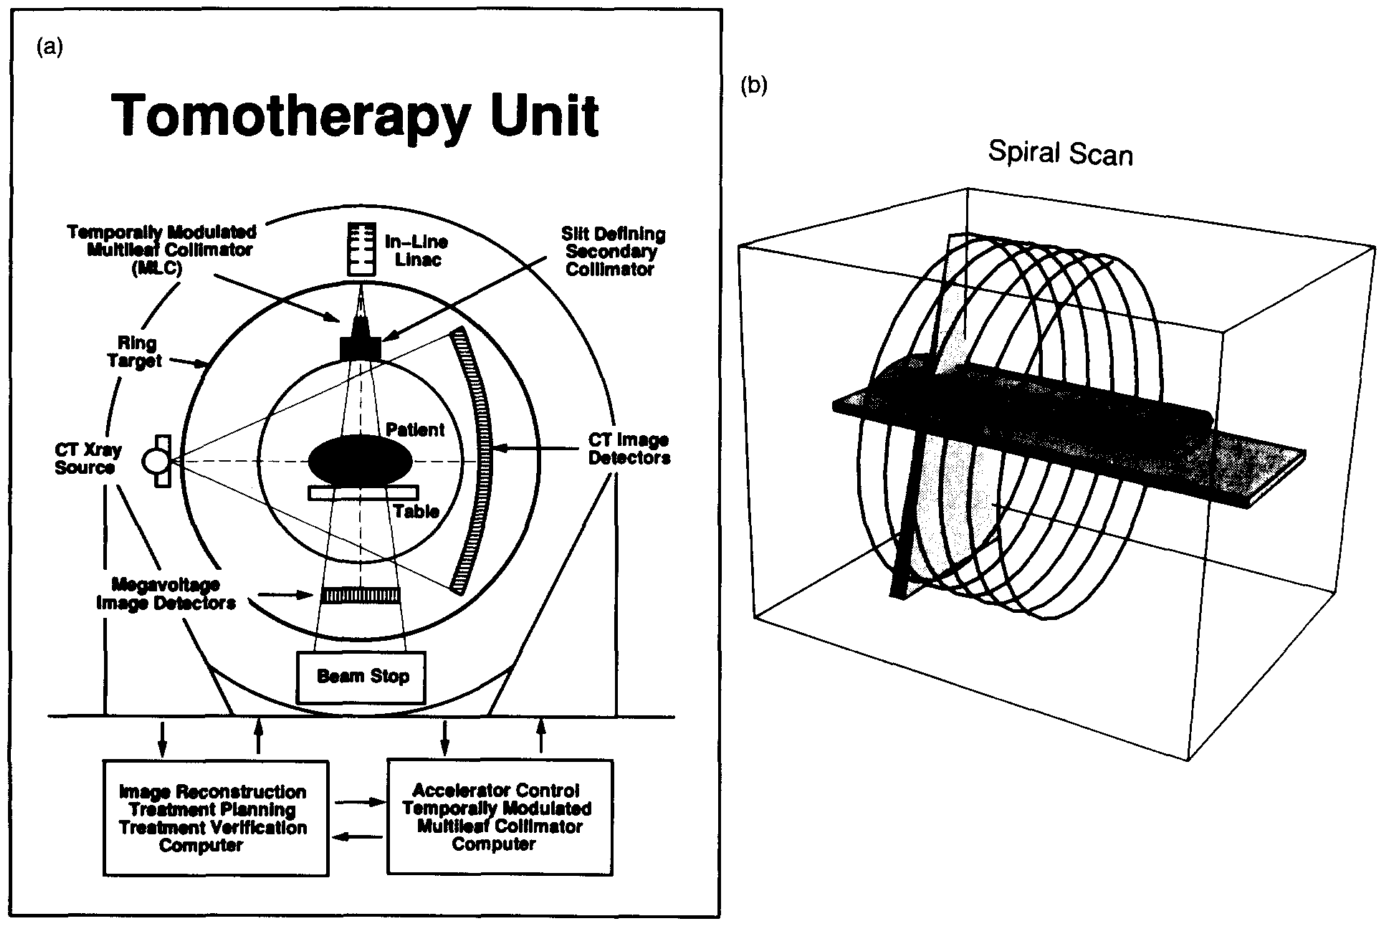
\includegraphics[width=\linewidth]{fig1}
  \label{fig1}
  \caption{A traditional tomotherapy unit, Ref \cite{Mackie1993}. (a) A block 
  diagram showing the ring gantry, and the radiation source}
  \end{figure*}
	%----------------------------------
	% References
  %----------------------------------
  
  \section{Methods and Materials}
  \subsection{Construction}
  \subsubsection{A note on Serial Tomotherapy}
  \subsection{Radiation Characteristics}
  \subsection{Comparisions between other conformal therapy techniques}
  \section{Clinical Results}
  \subsection{Whole brain helical Tomotherapy}
  \subsection{Inoperable Lung Cancer}
  \subsection{Rectal Cancer}
  
  \bibliography{Paper}{}
  \bibliographystyle{IEEEtran}
  
\end{document}